% AAMAS 2027 research paper draft.
% The official AAMAS 2027 class and layout are used without modification.
\documentclass[sigconf,anonymous]{aamas}

\graphicspath{{reference/template/}}
\usepackage{balance}
\usepackage{booktabs}
\usepackage{multirow}
\usepackage{array}
\usepackage{xspace}
\usepackage{enumitem}
\newcolumntype{P}[1]{>{\raggedright\arraybackslash}p{#1}}

\makeatletter
\gdef\@copyrightpermission{
  \begin{minipage}{0.2\columnwidth}
   \href{https://creativecommons.org/licenses/by/4.0/}{
\includegraphics[width=0.90\textwidth]{by}}
  \end{minipage}\hfill
  \begin{minipage}{0.8\columnwidth}
   \href{https://creativecommons.org/licenses/by/4.0/}{This work is licensed under a Creative Commons Attribution International 4.0 License.}
  \end{minipage}
  \vspace{5pt}
}
\makeatother

\setcopyright{ifaamas}
\acmConference[AAMAS 2027]{Proc.\@ of the 26th International Conference on Autonomous Agents and Multiagent Systems (AAMAS 2027)}{3--7 May 2027}{Hanoi, Vietnam}{M.~Baldoni, F.~Fang, W.~Yeoh, N.~Yorke-Smith (eds.)}
\copyrightyear{2027}
\acmYear{2027}
\acmDOI{}
\acmISBN{}
\acmSubmissionID{}
\submissionType{Research Paper Track}

\title{After the Decision: Learning to Adapt from Delayed Outcomes}
\author{Anonymous Authors}

\begin{abstract}
Scientific agents often choose among several tools that return plausible but conflicting answers. The challenge is not only selecting a provider before its output is visible: correctness feedback is produced after termination, may be delayed, and must update later choices without inventing labels for unselected tools. We present MIRA-Relay, an outcome-aware routing loop that combines a frozen discriminative provider surface with a lightweight provider-local residual adapter and an explicit release ledger. At cold start the adapter is exactly the frozen selector; after a selected result is released, it updates only that provider's residual reliability and can move the next action. We evaluate a one-call BBB routing contract with public truth, four checkpoint-bound fresh providers, scaffold-disjoint confirmation molecules, selected-only feedback, and delays $D\in\{0,1,4\}$. On the natural fresh holdout, MIRA-Relay matches Frozen at 89.81\% selected correctness; under a preregistered controlled evaluator-side label flip applied when the fit-best provider is selected, it reaches 87.56\% versus 73.38\% for Frozen, a +14.18-point paired gain with a 95\% scaffold bootstrap interval of [+9.61,+19.03] points. The result isolates the claim: delayed selected-only feedback supports recovery from the declared drift, while a stationary fresh menu does not justify a generic online gain.
\end{abstract}

\ccsdesc[500]{Computing methodologies~Multi-agent planning}
\ccsdesc[300]{Computing methodologies~Reinforcement learning}
\ccsdesc[200]{Computing methodologies~Machine learning}
\keywords{tool selection, online learning, delayed feedback, scientific agents, molecular property prediction}

\newcommand{\mira}{MIRA-Relay\xspace}
\begin{document}
\maketitle

\section{Introduction}
A scientific agent must decide which tool's prediction to use when several providers estimate the same property. That choice matters even when every call completes: execution success establishes that an answer was returned, while usefulness depends on whether the answer is correct for the input. Molecular property prediction makes this distinction measurable because provider outputs can be checked against independently recorded endpoint labels.

Valid responses can disagree on the same molecule. In our frozen BBB development panel, molecule \texttt{z000282} has benchmark label $1$: \texttt{admet\_ai\_1\_4\_0} returns $0$, while \texttt{b3clf\_dtree\_common} returns $1$, both with successful runtime status. The example establishes a selection problem; it does not establish which provider is best on the next molecule. During evaluation, the agent sees neither unselected outputs nor the current correctness label before choosing.

Outcome feedback creates two obstacles: sparse coverage and delayed release. A fixed policy cannot use new evidence. A selected-only learner sees feedback only from chosen providers, leaving alternatives sparsely observed; delay postpones when feedback is usable. These constraints motivate our adaptation hypothesis but do not prove that any bandit fails. We therefore compare matched online controls and test whether released provider-local evidence changes later decisions.

We hypothesize that a released outcome can inform later choices through a shared released state. Each provider keeps its own residual, so the update need not assume that providers are independent or interchangeable. An immutable fit-time reference anchors the comparison. The claim requires a change in later exploitation under identical observations.

MIRA-Relay is the concrete instantiation of this hypothesis within the MIRA adaptation framework. Its cold-start surface is frozen, while a selected-only reliability ledger adds a provider-specific residual only after the corresponding outcome is released. The residual is centered on that provider's fit-time success rate, so the adapter starts exactly at the frozen policy and changes only when released evidence is strong enough to move a later ranking. Runtime failure, unknown truth, and chemical error remain separate ledger fields. A post-call verifier is a defined extension interface; the paper's primary claim is the one-call routing contract.

This draft makes four testable commitments, each paired with a falsification condition in the experimental matrix:
\begin{itemize}[leftmargin=*,itemsep=1pt,topsep=2pt]
    \item \textbf{Task validity.} Public truth and a concrete provider panel yield input-dependent headroom over a fixed provider without leaking unselected outcomes; this fails if an evaluator-only panel score is the only source of signal.
    \item \textbf{Faithful adaptation.} Selected-only delayed events can be replayed with exact visibility, release clocks, and failure semantics; this fails if the contract/replay checks cannot validate the recorded action and release sequence.
    \item \textbf{Mechanistic adaptation.} Released outcomes alter later choices beyond matched controls; this fails if changes cannot be traced to selected-only events.
    \item \textbf{Practical value.} Any improvement in future correctness must survive the strongest legal fixed and matched online controls while reporting harmed decisions, calls, latency, and memory; otherwise the conclusion is limited to a protocol or diagnostic result.
\end{itemize}
The remainder of the paper defines the task, gives the proposed specification, fixes the benchmark and baseline contracts, and reports the natural fresh-menu confirmation together with a preregistered correctness-drift stress.

\begin{figure*}[t]
  \centering
  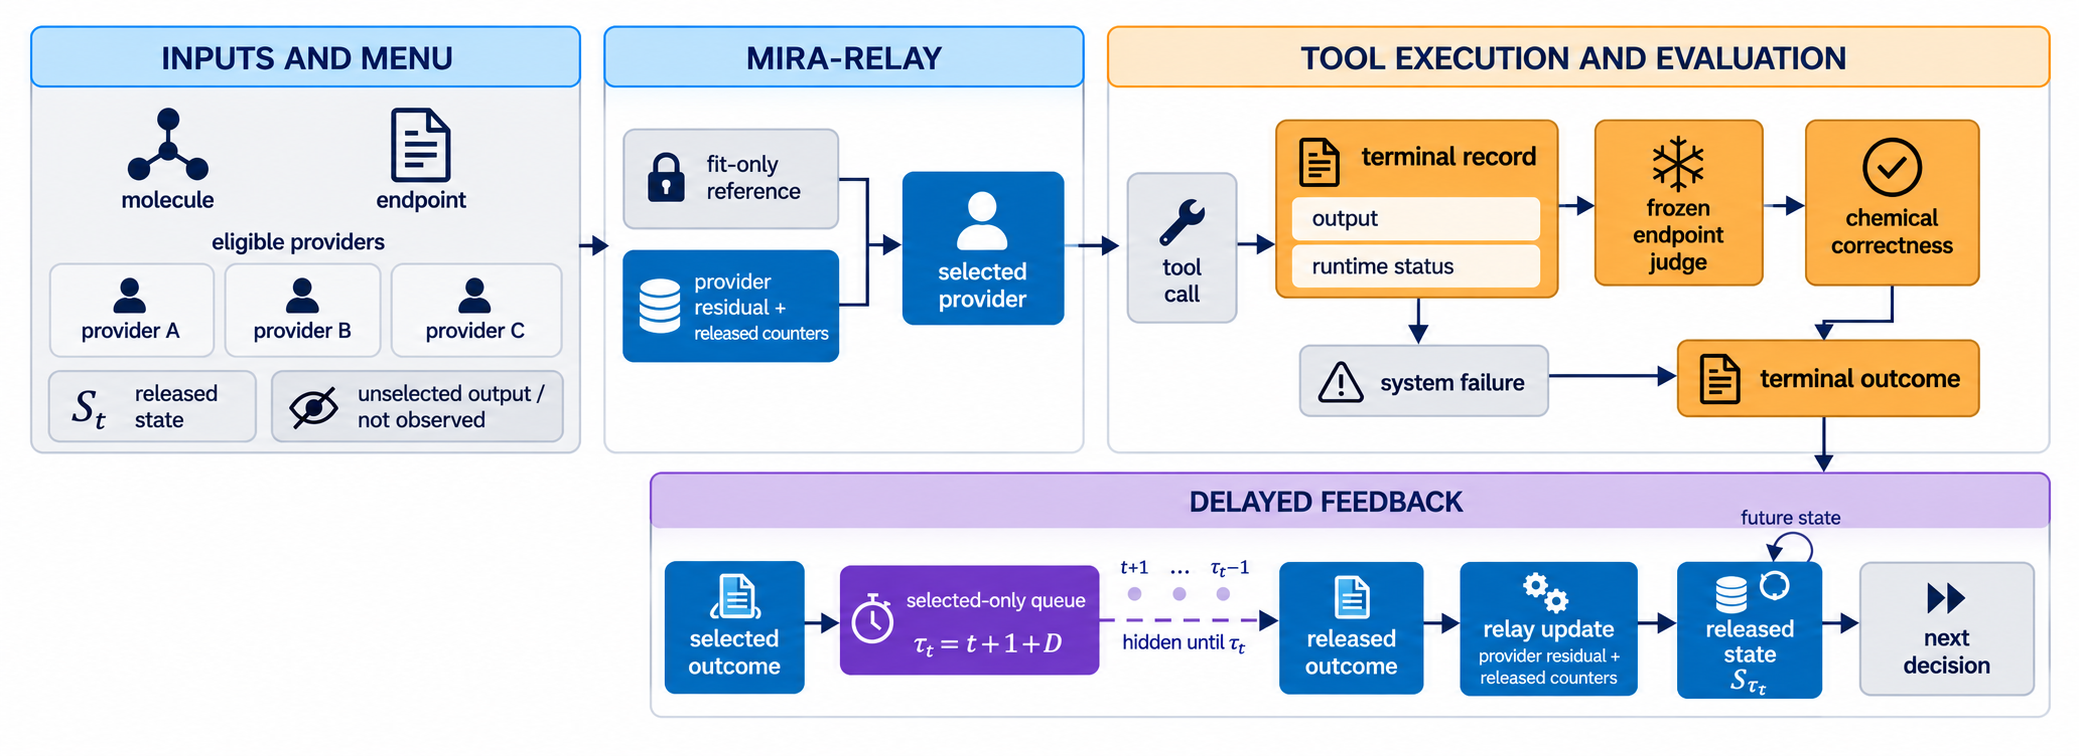
\includegraphics[width=\textwidth]{figures/generated/figure1/v05_ai.png}
  \caption{MIRA-Relay closes the loop from a pre-call choice to a later decision. Molecule, endpoint, eligible menu, and released state enter a frozen provider surface plus a provider-local residual ledger. One selected call produces a terminal record; the frozen endpoint judge supplies chemical correctness only after termination, while runtime failure follows its own ledger. The selected outcome waits until $\tau_t=t+1+D$ and then updates the released state; decisions continue while feedback is pending.}
  \Description{A four-region full-width architecture: inputs and eligible providers enter MIRA-Relay, which combines an immutable fit-only provider surface with a selected-only provider residual ledger to select one provider. The call creates a terminal record with output and runtime status; a frozen endpoint judge produces chemical correctness after termination, and runtime failure enters a runtime ledger. The selected outcome waits in a delayed queue until tau equals t plus one plus D, updates the released state, and feeds the next decision.}
  \label{fig:overview}
\end{figure*}

\section{Problem and Task Contract}
We study one agent making a sequence of tool calls. Figures~\ref{fig:overview} and~\ref{fig:lifecycle} show the same contract at two scales: the first separates the learned relay from execution and evaluation, while the second fixes the event order that determines when feedback can affect a later action. The contract is defined at the granularity of a concrete provider, not a provider family or a post-hoc majority vote.

\subsection{Episode, menu, and feedback}
At decision tick $t$, the agent receives a molecule $x_t$, an endpoint $e_t$, and an available menu $A_t$ of concrete provider identifiers. It chooses one provider $a_t\in A_t$ before reading the current output panel. The benchmark stores an independent endpoint truth $y_t\in\{0,1\}$ for evaluation. The selected call returns an output $o_t$, a runtime status $s_t\in\{\mathrm{ok},\mathrm{error}\}$, and, when available, a confidence value $c_t$. We keep the labels that drive the method separate:
$$
\begin{aligned}
 r_t^{\mathrm{run}}&=\mathbf{1}[s_t=\mathrm{ok}],\\
 r_t^{\mathrm{chem}}&=\begin{cases}\mathbf{1}[o_t=y_t],&s_t=\mathrm{ok},\\ \mathrm{null},&s_t=\mathrm{error},\end{cases}\\
 r_t^{\mathrm{sys}}&=\mathbf{1}[s_t=\mathrm{ok}\land o_t=y_t].
\end{aligned}
$$
The correctness head is trained only on non-null $r^{\mathrm{chem}}$; the runtime head uses $r^{\mathrm{run}}$; a bandit reward may use $r^{\mathrm{sys}}$ with separate failure and chemical-error costs. Thus an execution failure is not silently relabeled as a chemical mistake.

After termination, a replay judge records the selected outcome. The outcome becomes visible only at its registered release tick $\tau_t$. The legal history at tick $t$ is
$$
H_t=\{(x_s,e_s,a_s,r_s^{\mathrm{sys}},\tau_s):s<t,\ \tau_s\leq t\}.
$$
For example, for molecule \texttt{z000282}, the benchmark truth is $1$. The call to \texttt{admet\_ai\_1\_4\_0} returns $0$ with status `ok`. The call to \texttt{b3clf\_dtree\_common} returns $1$ with status `ok`. Both calls have $r^{\mathrm{run}}=1$, but their chemical labels differ. A decision at tick 2 cannot read either unselected output, the current truth, or any future terminal record.

Provider parameters use a registry $\mathcal P$ fixed at initialization; $A_t\subseteq\mathcal P$ is the current candidate menu. Removing a challenger leaves its stored state intact. For the historical BBB replay, $|\mathcal P|=33$ throughout the stream. The queue orders releases by due tick and breaks ties by enqueue order; each feedback is consumed once and receipts record the release order explicitly.

For the fixed-delay replay, a decision at tick $t$ terminates, enqueues its feedback, and releases it at
$$
\tau_t=t+1+D,\qquad D\in\{0,1,4\}.
$$
Only after this release may the event enter $H_{t'}$ and affect a later decision. For $D=0$, the release is processed before the next decision tick and never changes the action that caused the event. Unknown truth creates no correctness label and stops the current scoring stream; a refusal creates no selected-provider label. Both remain explicit in the episode ledger.

\subsection{Selection and verification interfaces}
The pre-call selector and post-call verifier have disjoint interfaces:
$$
a_t=\pi_{\mathrm{sel}}(x_t,e_t,A_t,H_t,S_t),\qquad v_t=\pi_{\mathrm{ver}}(o_t,c_t,s_t),
$$
where $v_t$ is one of accept, escalate, or refuse. The verifier can request a second provider only after the first call returns. This is an extension interface for E5, not an action performed by the current direct-selection runner. In the running example, a selector may choose `b3clf\_dtree\_common`; only after its output and confidence are available can the verifier decide whether to escalate.

The online learner maintains a serializable post-release state $S_t$. At tick $t$, the release phase first applies exactly the events due at that tick; the selector then reads the resulting state:
$$
\begin{aligned}
S_t&=U\left(S_{t-1},\right.\\[-2pt]
&\qquad\left.\{(x_s,e_s,a_s,r_s^{\mathrm{sys}},\tau_s):s<t,\ \tau_s=t\}\right),\\
a_t&=\pi_{\mathrm{sel}}(x_t,e_t,A_t,H_t,S_t).
\end{aligned}
$$
With no due event, $U$ is the identity. Thus a $D=0$ event from tick $t$ enters $S_{t+1}$ and can affect action $t+1$, but never action $t$.
No correctness-residual update is allowed for an unselected provider, an unreleased event, an unknown label, or a refusal. A terminal unknown or refusal may still update runtime/availability bookkeeping; every selected scored provider, including the fit-best provider, receives only its own released residual update. This contract lets a receipt verifier check the visible read set, action, release queue, recorded state fields, and schema/counts. Complete metric recomputation is left to the E5 transition replayer; this receipt check does not by itself recompute scores, propensities, or the update.

\subsection{Estimands and costs}
The primary estimand is prequential system success: a selected call must return a valid and correct answer. We also report chemical correctness conditional on valid returns, paired rescued and harmed decisions, failures, and call and update costs. The extension interface additionally accounts for escalation, refusal, and unknown truth; those utilities are outside the reported one-call result. Static full-panel accuracy and an evaluator-only retrospective best-fixed control measure task headroom separately from online effects.

\section{MIRA-Relay: Proposed Method Specification}
This section specifies MIRA-Relay and the information boundary tested in the one-call experiments.

\subsection{Cold-start scores and the immutable reference}
Let $\phi(x)\in\mathbb{R}^{d}$ be a frozen molecule representation and let $K=|\mathcal P|$ be the number of concrete providers. For each provider $a$, a logistic correctness head $w_a^0$ is fitted once on the fit partition. Its cold-start score is
$$
q_a^0(x)=\sigma\!\left((w_a^0)^\top\phi(x)\right).
$$
The current menu only masks which coordinates can act; no current output is read before the action. For the fresh BBB confirmation, $d=65$: 64 Morgan bits plus an intercept. The fit-only Best Fixed provider is the provider with the highest fit-partition correctness. The frozen base scores are immutable throughout evaluation, and every provider switch is still counted even when it is wrong.

The running case is concrete. For molecule \texttt{z000282}, $\phi(x)$ is the frozen 65-dimensional vector built from its canonical SMILES and the intercept; the fit heads assign separate scores to the four fresh providers. At cold start, MIRA-Relay and Frozen therefore choose the same provider for the same menu. Providers outside the sealed checkpoint manifest are out of scope.

\subsection{Context-relative reliability adapter}
For provider $a$, let $\bar r_a$ be its fit-partition correctness rate and let $n_{a,t}$ and $s_{a,t}$ be, respectively, the number of its selected outcomes released by tick $t$ and the number that were correct. With a fixed prior count $n_0=20$, the released posterior rate and residual are
$$
\widehat r_{a,t}=\frac{n_0\bar r_a+s_{a,t}}{n_0+n_{a,t}},\qquad
\Delta_{a,t}=\widehat r_{a,t}-\bar r_a.
$$
The action score is
$$
q_{a,t}(x)=q_a^0(x)+\Delta_{a,t},
\qquad
 a_t=\arg\max_{a\in A_t}q_{a,t}(x_t).
$$
At cold start, $n_{a,0}=s_{a,0}=0$ and therefore $\Delta_{a,0}=0$: the adapter is exactly Frozen. When a selected outcome becomes visible, only that provider's counters change; an unselected provider never receives a synthetic label. A runtime error is recorded as an execution failure and is not inserted into the chemical-correctness count. This provider-local residual is added to the $x$-conditioned frozen score. Here ``context-relative'' refers to the current provider ranking and released evidence state, not to a second $x$-conditioned head; the fit-time representation itself never changes.

The case makes the update concrete. If the selected provider for \texttt{z000282} is correct, $s_{a,t}$ and $n_{a,t}$ each increase by one at its release tick. If it is wrong, only $n_{a,t}$ increases. The next score changes by the corresponding residual; all unselected providers keep their previous residuals. The update is $O(1)$ per released event and scoring is $O(Kd)$, while the online ledger stores $2K$ counters and the fixed heads remain outside the online state.

\subsection{Bounded evidence interface}
The same selector can be extended after the first call. Let $E_t$ denote the returned output and runtime record. A verifier may accept, refuse, or request one additional provider call by minimizing a declared loss that includes call cost and refusal cost. This interface is specified so that a future evidence experiment has a fixed action vocabulary; it is outside the primary one-call result reported here.

\subsection{Release ledger and delayed update}
The online state is the selected-only ledger $S_t=\{(n_{a,t},s_{a,t}) : a\in\mathcal P\}$. At tick $t$, the release queue first applies every event with due time $\tau=t$; the selector then reads the resulting state. For a fixed delay,
$$
\tau_t=t+1+D,\qquad D\in\{0,1,4\}.
$$
Thus a $D=0$ event from tick $t$ can affect action $t+1$, never action $t$. The state transition is deterministic given the released event prefix, which makes the receipt replayable from recorded evidence.

The update touches only the selected provider. For a scored terminal record $s$ released at tick $t=\tau_s$, with chemical label $r_s^{\mathrm{chem}}\in\{0,1\}$,
$$
 n_{a_s,t}^{+}=n_{a_s,t}^{-}+1,\qquad
 s_{a_s,t}^{+}=s_{a_s,t}^{-}+r_s^{\mathrm{chem}},
$$
where $-$ and $+$ denote the state immediately before and after the queue applies that release; all other provider counters are unchanged. If the call fails, $r^{\mathrm{chem}}$ is null and the runtime-failure ledger records the event separately. Unknown truth and refusal do not update correctness counters. This separation is the central information boundary: the learner receives exactly the selected outcome after release, never the current truth or an unselected provider's output.

The update is $O(1)$ per released event and scoring all $K$ providers costs $O(Kd)$. The online state uses $2K$ counters plus masks and the release queue. For \texttt{z000282}, a released result changes one provider residual, so the next action can switch according to the evidence.

\begin{figure*}[t]
  \centering
  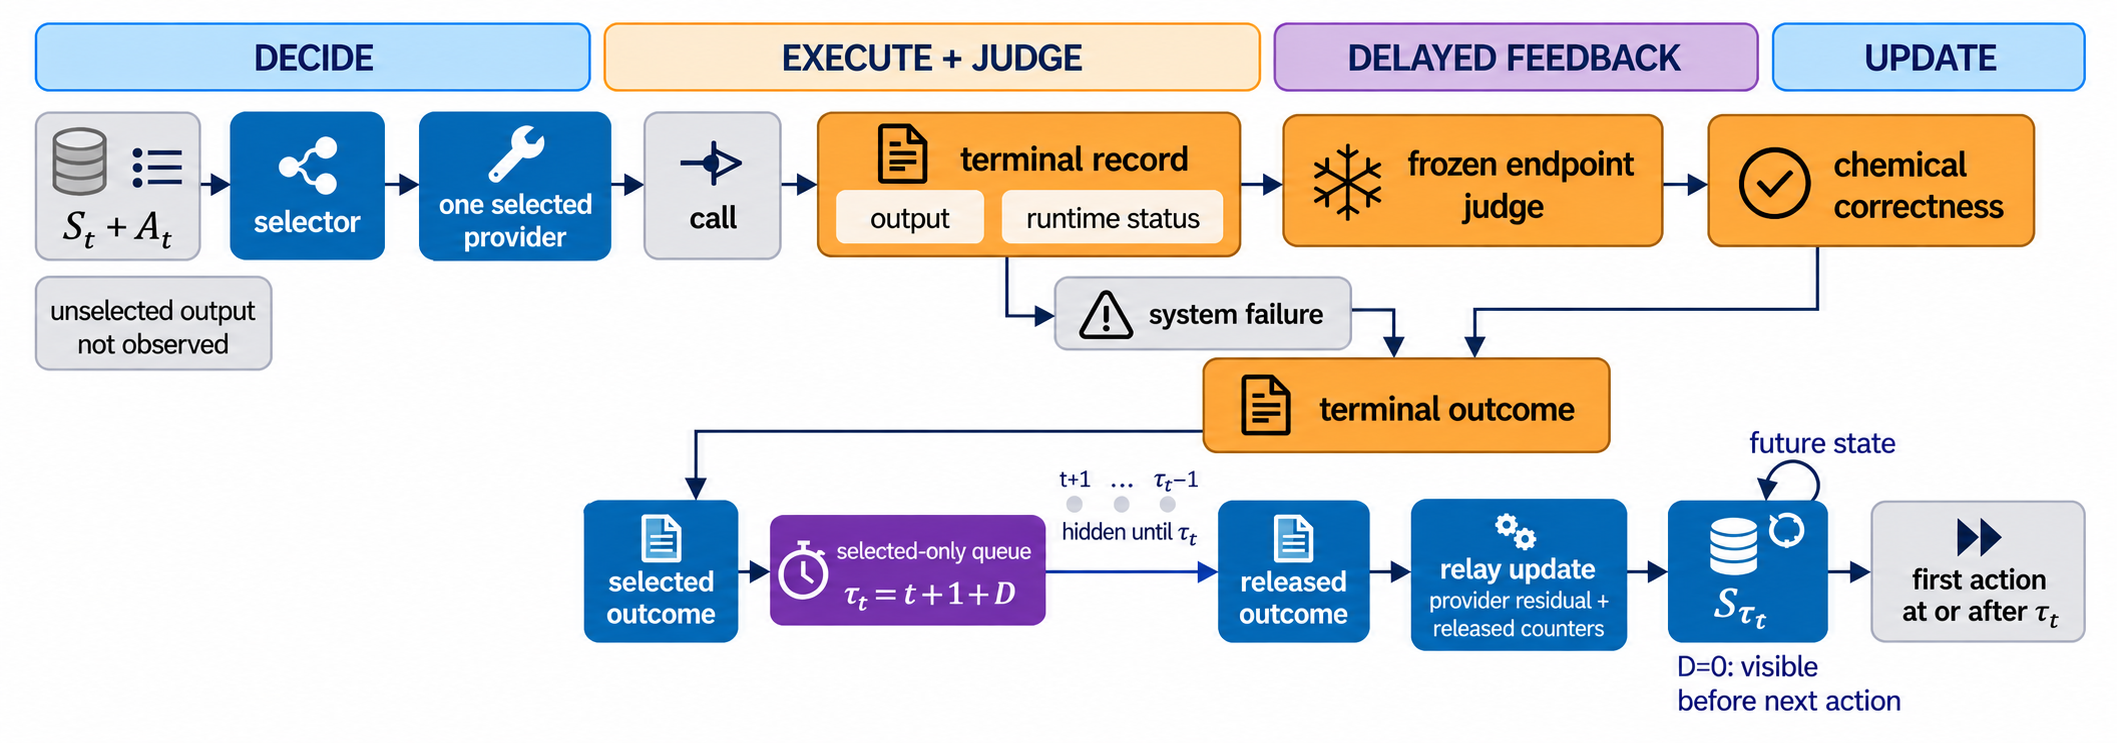
\includegraphics[width=\textwidth]{figures/generated/figure2/v22_ai.png}
  \caption{The terminal feedback contract. At decision tick $t$, the selector sees $S_t$ and $A_t$ and chooses one provider before any current output is observed. The terminal record is split into output and runtime status; the frozen endpoint judge then yields chemical correctness only after termination. Runtime failure and chemical correctness form the selected terminal outcome, which waits in a selected-only queue until $\tau_t=t+1+D$. The relay update is visible to the first action at or after release; for $D=0$, this is the next action.}
  \Description{A full-width event flow from state and menu to selector, one selected provider, call, terminal record, frozen endpoint judge, chemical correctness, runtime failure, and terminal outcome. The selected outcome enters a selected-only queue, remains hidden until tau equals t plus one plus D, then updates the relay and released state before the next action. An eye-slash marks unselected output as unobserved.}
  \label{fig:lifecycle}
\end{figure*}

\subsection{Action rule and falsification}
The primary one-call runner uses the highest current score in the eligible menu. There is no result-dependent probe in the reported fresh confirmation, so every method receives the same one-call budget and the same selected-only feedback clock. The controlled stress flips the selected label of the fit-best provider after the preregistered midpoint; it does not reveal any unselected output or alter the input features.

The implementation preserves five invariants: (i) no current truth or unselected output is read before action, (ii) only released selected events update state, (iii) the fit surface is immutable, (iv) runtime failure and chemical correctness remain separate, and (v) the released event prefix determines the next action. The receipt records a learned-state snapshot, release queue, action, and event schema; an independent receipt checker validates the exact event identities and order, selected correctness, release clocks, and opaque state-hash/version continuity. The older receipt does not contain enough state bytes to rehash a learned policy independently.

The adaptive claim is rejected if the residual cannot change a later action under the declared drift, if contract/replay checks find a mismatch, or if the gain disappears against the same-schedule Frozen and matched Online-SGD controls. Action changes alone are not treated as utility; the evaluation reports rescued and harmed decisions, scaffold-cluster intervals, calls, and update latency.

\section{Benchmark and Baselines}
\subsection{Two-layer benchmark contract}
The benchmark has a public truth layer and a provider-routing layer. The truth layer uses the Therapeutics Data Commons (TDC) BBB endpoint, fixed label semantics, and its split archive~\cite{huang2021tdc}. The development manifest contains 722 labeled molecules; 716 have complete outputs from the 33-provider Task36 panel. Conflict groups are excluded under the project decision, with raw receipts retained for audit. Because the old panel overlaps the official BBB test (147 canonical molecules; 235 scaffolds), it is not an untouched confirmation set.

The routing layer turns cached outputs into sequential decisions with a fixed registry, eligible-menu mask, selected-only feedback, delayed release, and explicit failures. It is a project protocol grounded in public truth. The fresh study keeps four checkpoint-bound providers; the wider 33-provider pool is development evidence, not a model-fresh claim. Unknown truth stops a single-call stream, while verification, refusal, provider arrival, hERG, and AMES use separate extension contracts.

\subsection{Baselines and fairness}
Table~\ref{tab:baselines} groups the deployable comparators by the role they play in the routing question. Every method receives the same molecule, endpoint, menu, fit-only initialization, selected-only feedback, delay, and one-call budget. Full-panel labels are used only for fit warm starts or evaluator-only controls.

\begin{table}[t]
\caption{Comparator groups under the common routing contract.}
\label{tab:baselines}
\footnotesize
\begin{tabular}{@{}P{0.22\linewidth}P{0.34\linewidth}P{0.34\linewidth}@{}}
\toprule
Role & Methods & Purpose \\
\midrule
Anchors & Random; Best Fixed; Retrospective Best Fixed$^{\dagger}$ & blind, fit-only and evaluator-only references \\
Frozen / matched updates & Frozen; MIRA-Relative; Online SGD & isolate the value of a released update \\
Modern online controls & Greedy LinUCB; BayesianRouter & current contextual and posterior controls \\
Proposed & MIRA-Relay & selected-only provider residual under delay \\
\bottomrule
\end{tabular}
\begin{flushleft}
\footnotesize $^{\dagger}$Evaluator-only retrospective control; it is not a deployable baseline.
\end{flushleft}
\end{table}

Recent routers with incompatible input or feedback semantics remain audit-only. PILOT, GraphRouter, RouterDC, and RouterBench need a separate wrapper and leakage audit; our result covers the sealed four-provider menu, not 33-provider or model-fresh generalization.

\section{Experiments}
We use a public BBB truth layer and a sealed four-provider fresh menu. The fit partition is scaffold-disjoint from 157 confirmation molecules; each policy sees only the molecule features, endpoint, eligible menu, and released selected outcomes. We evaluate five folds, two seeds, and delays $D\in\{0,1,4\}$ under a one-call budget. The matrix and intervention were frozen before confirmation runs; the full event contract and hyperparameters are in the artifact. Table~\ref{tab:matrix} is the experimental map.

\begin{table*}[t]
\caption{Experimental map. Each row answers one question; all online rows use the same 157-molecule fresh menu and selected-only release clock unless stated otherwise.}
\label{tab:matrix}
\footnotesize
{\setlength{\tabcolsep}{2pt}
\begin{tabular}{@{}P{0.15\linewidth}P{0.25\linewidth}P{0.34\linewidth}P{0.14\linewidth}@{}}
\toprule
Question & Data / intervention & Compared methods & Primary metric \\
\midrule
Headroom & 722 BBB development molecules; scaffold-fold fit/validation & Random, Best Fixed, Frozen & OOF selected correctness and headroom \\
Natural adaptation & 157 fresh molecules; $D\in\{0,1,4\}$; no label flip & Frozen, MIRA-Relative, MIRA-Relay, Online SGD, Greedy LinUCB, BayesianRouter & prequential correctness, paired scaffold CI, latency \\
Drift recovery & Same fresh menu; selected fit-best label flips after tick 78 & Frozen, Online SGD, Greedy LinUCB, BayesianRouter, MIRA-Relay & recovery correctness, rescued/harmed switches \\
Cost / validity & All confirmation streams & All one-call methods & calls, failures, replay checks, p95 update time \\
\bottomrule
\end{tabular}}
\end{table*}

Rows 1--3 test headroom, stationary adaptation, and a midpoint label flip. The last row checks calls and replay under the same release clock. Verification, refusal, lifecycle, hERG, and AMES are separate extensions.

\section{Results}
The primary confirmation contains 270 natural streams and 150 controlled-drift streams. Every stream has 157 decisions and one provider call per decision; all reported intervals are scaffold-cluster bootstrap intervals.

\begin{table}[H]
\vspace{-6pt}
\caption{Natural fresh-menu confirmation across 157 scaffold-disjoint molecules. Success is the mean over 4,710 paired calls; intervals resample Bemis--Murcko scaffold clusters after aggregating repeated schedules. Update p95 is CPU policy-operation overhead on macOS arm64, excluding I/O and provider inference.}
\label{tab:main-results}
\footnotesize
{\setlength{\tabcolsep}{2.0pt}
\begin{tabular}{@{}P{0.24\linewidth}P{0.13\linewidth}P{0.38\linewidth}P{0.15\linewidth}@{}}
\toprule
Method & Success & Paired $\Delta$ (95\% CI) & Update p95 \\
\midrule
Random & 83.76\% & -6.05 pp [-9.93,-2.26] & $5.44\,\mu\mathrm{s}$ \\
Best Fixed & 88.15\% & -1.66 pp [-3.97,+0.51] & $0.68\,\mu\mathrm{s}$ \\
Frozen & 89.81\% & 0 & $1.31\,\mu\mathrm{s}$ \\
MIRA-Relative & 89.81\% & 0.00 pp [0.00,0.00] & $73.30\,\mu\mathrm{s}$ \\
MIRA-Relay & 89.81\% & 0.00 pp [-1.24,+1.40] & $2.81\,\mu\mathrm{s}$ \\
Online SGD & 89.21\% & -0.59 pp [-1.80,+0.52] & $19.37\,\mu\mathrm{s}$ \\
Greedy LinUCB & 89.72\% & -0.08 pp [-0.58,+0.41] & $90.90\,\mu\mathrm{s}$ \\
BayesianRouter & 89.53\% & -0.28 pp [-1.75,+0.97] & $88.96\,\mu\mathrm{s}$ \\
Retrospective Best Fixed$^{\dagger}$ & 90.45\% & +0.64 pp [-2.86,+4.07] & $0.54\,\mu\mathrm{s}$ \\
\bottomrule
\end{tabular}}
\begin{flushleft}
\footnotesize $^{\dagger}$Evaluator-only fixed provider chosen after observing confirmation labels; it is a headroom reference, not an oracle or deployable policy.
\end{flushleft}
\end{table}

\paragraph{Natural fresh menu.} We ask whether released selected outcomes improve a stationary fresh menu. Table~\ref{tab:main-results} shows that Frozen is within 0.64 points of the retrospective best-fixed reference. MIRA-Relay changes 164 actions, rescuing and harming 82 decisions each, so its 89.81\% accuracy is identical to Frozen (paired $\Delta=0.00$ points, 95\% CI $[-1.24,+1.40]$). The BayesianRouter, Greedy LinUCB, and matched SGD controls have paired differences from Frozen whose intervals span zero. The stationary result is therefore a stability check, not evidence for a generic online gain.

\begin{table}[H]
\vspace{-6pt}
\caption{Controlled correctness-drift stress. Success is pooled over 4,710 paired calls. Changes count post-release action changes relative to Frozen; rescued/harmed counts are relative to the same-receipt Frozen action. Paired intervals resample scaffold clusters.}
\label{tab:mechanism-results}
\footnotesize
{\setlength{\tabcolsep}{1.0pt}
\begin{tabular}{@{}P{0.19\linewidth}P{0.12\linewidth}P{0.09\linewidth}P{0.12\linewidth}P{0.18\linewidth}P{0.23\linewidth}@{}}
\toprule
Method & Success & $N$ & Changes & Rescued / harmed & Paired $\Delta$ (95\% CI) \\
\midrule
Frozen & 73.38\% & 4710 & 0 & -- & -- \\
Matched SGD & 84.03\% & 4710 & 2566 & 720 / 218 & +10.66 pp [+6.05,+15.45] \\
Greedy LinUCB & 81.15\% & 4710 & 874 & 414 / 48 & +7.77 pp [+5.08,+10.72] \\
BayesianRouter & 80.28\% & 4710 & 1654 & 492 / 167 & +6.90 pp [+3.50,+10.41] \\
MIRA-Relay & 87.56\% & 4710 & 1884 & 780 / 112 & +14.18 pp [+9.61,+19.03] \\
\bottomrule
\end{tabular}}
\end{table}

\paragraph{Controlled drift recovery.} In the preregistered stress, the evaluator flips the selected fit-best provider's label after tick 78 without changing features, menus, or feedback visibility. Table~\ref{tab:mechanism-results} shows that MIRA-Relay reaches 87.56\% versus 73.38\% for Frozen, a +14.18-point paired gain (95\% CI $[+9.61,+19.03]$). Matched SGD, Greedy LinUCB, and BayesianRouter recover by +10.66, +7.77, and +6.90 points; the Bayesian interval is $[+3.50,+10.41]$. Across $D=0,1,4$, the paired gain over Frozen is $+13.63,+14.52,+14.39$ points; the natural differences are $-0.13,-0.13,+0.25$ points. The result is a response to the declared drift, not a claim about natural provider nonstationarity. All 420 streams pass contract/replay verification, and no method uses more than one provider call per molecule. The artifact retains the evidence-extension and lifecycle protocols, but they are not reported as empty tables.

\begin{figure*}[t]
  \centering
  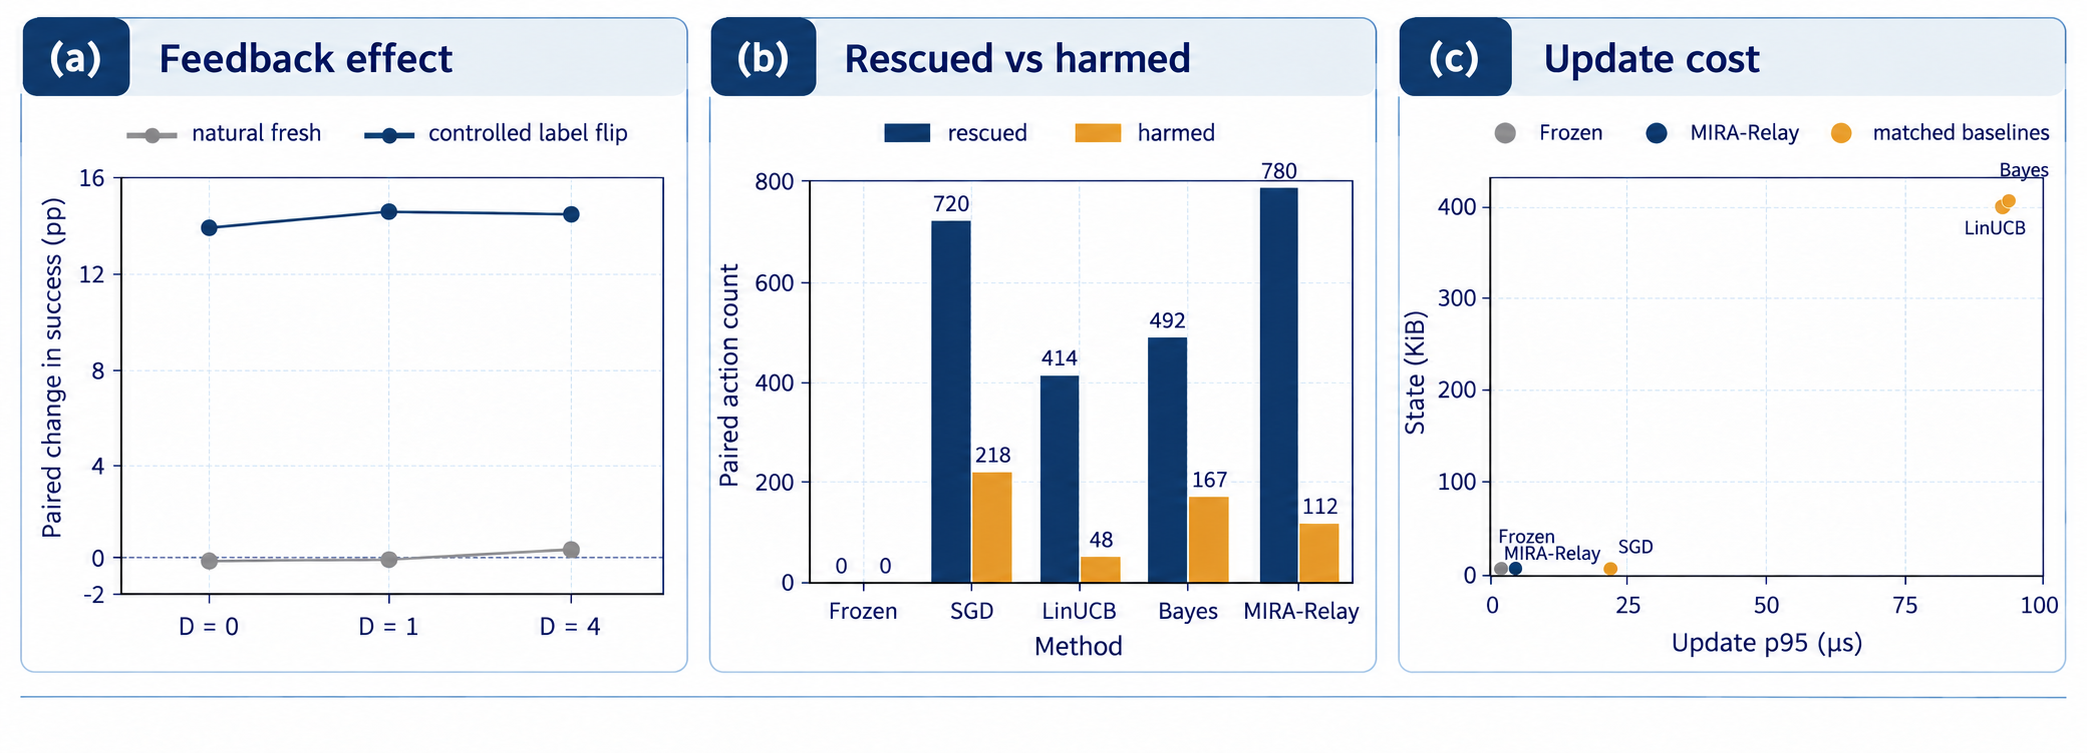
\includegraphics[width=\textwidth]{figures/generated/figure3/v05_ai.png}
  \caption{Receipt-bound evidence views for the three-figure confirmation. Panel (a) reports paired success changes relative to Frozen under natural fresh feedback and the controlled label-flip stress across release delays. Panel (b) counts rescued and harmed actions against the same-receipt Frozen action. Panel (c) shows policy-update p95 against serialized online state for Frozen, MIRA-Relay, and matched baselines.}
  \Description{Three compact result panels: feedback effect across delays, rescued versus harmed action counts for five methods, and update p95 versus serialized state for Frozen, MIRA-Relay, and matched baselines.}
  \label{fig:evidence}
\end{figure*}

\section{Error and Cost Analysis}
We report errors by provider, scaffold group, runtime status, and feedback visibility. A wrong terminal prediction, a provider execution failure, an unknown truth, and an intentional refusal are different events and remain in separate denominators. The current fresh receipt reports selected correctness, rescued/harmed switches, calls, and update timing; the post-call utility decomposition is reserved for the out-of-scope evidence extension. This separation is necessary because a small pooled accuracy change can hide a large number of harmful switches.

The receipt reports calls, serialized state, replay checks, and update p95. Timing measures policy computation; it excludes file I/O, provider inference, evaluator scoring, and service latency. Across the 270 natural streams, MIRA-Relay update p95 is $2.813\,\mu\mathrm{s}$; in the 150-stream stress it is $3.464\,\mu\mathrm{s}$ under the same policy-operation timer. Every stream has 157 calls, and all 420 streams pass contract/replay checks. These are policy costs, not end-to-end service latency. Post-call verification is outside scope.

\section{Mechanism Interpretation}
The two fresh-menu results separate two questions that are often conflated in online routing. The first is whether a provider-specific adapter can change its action after observing a selected result. The second is whether the current provider panel contains a predictable opportunity for that change to improve accuracy. MIRA-Relay changes actions in the stationary confirmation, but the 82 rescued and 82 harmed decisions cancel at the aggregate level. This is the expected behavior of a conservative residual: it is allowed to react to evidence without being credited for a gain that the panel does not contain.

The controlled stress answers the first question directly. At the midpoint, the evaluator flips the returned label only when the fit-best provider is selected. The selector is not told the flip time, the affected provider, or the counterfactual outputs of alternatives. After the delay, released failures accumulate against that provider's residual, and later actions move to providers whose frozen scores are lower but whose observed evidence is now relatively better. Frozen cannot respond because its score surface is immutable. Matched Online-SGD, Greedy LinUCB, and BayesianRouter also respond, which is why they are reported as positive controls rather than straw baselines; MIRA-Relay's larger recovery is the result that must survive the common clock and the same feature surface.

The mechanism has a deliberately narrow interpretation. The residual is not a new endpoint predictor and it does not infer a hidden label for an unselected provider. It is a small correction to the fit-time score, centered on the provider's own fit rate. This centering matters in the selected-only setting: an uncentered success count would favor providers that are sampled more often, while a global multiplier would leave an argmax unchanged or change every provider in the same direction. The release ledger makes this distinction observable by recording the provider, due tick, state version, and action sequence for every event.

Three diagnostic comparisons are therefore reported together. Frozen measures the value of the fit-time surface alone. MIRA-Relay measures the added value of released selected evidence. MIRA-Relative is a stopped negative variant whose global reliability factor produces the same action sequence as Frozen on the natural fresh menu. The stress control shows that the positive result is not an artifact of merely having an update field: removing the update path leaves the degraded fit-best provider selected throughout the post-flip segment. The resulting interpretation is an adaptive capability with a measured boundary, rather than a claim that any online update improves a stationary panel.

\section{Limitations and Discussion}
The benchmark separates public answer semantics from the project routing protocol. This makes the provider-selection question replayable, but it does not make the routing layer a community benchmark by itself. The principal development endpoint is BBB; hERG and AMES remain extensions until their assay semantics, coverage, conflicts, and provider training lineage are closed. The current provider panel also contains related model families, so provider-count improvements cannot be interpreted as independent evidence without family-balanced analysis.

The proposed method is scoped to feedback-adaptive selection. A delayed selected-only replay does not by itself demonstrate natural provider arrival, retirement, version drift, or broad nonstationarity. Those events are controlled stress unless an independent deployment trace supports a stronger claim. The immutable frozen base is a reference and guardrail, not a theorem that no switch can be harmful.

The method may fail when selected feedback is too sparse, when a residual update is too small to change the next choice, or when a provider error transfers to a later decision. These alternatives motivate exposure, score-margin, and rescued/harmed analyses. A failed candidate remains evidence for revising the mechanism; it does not establish the project's target improvement or justify replacing that target with a protocol-only conclusion.

\section{Validity and Reproducibility Checks}
The confirmation is separated from the development diagnostic at three points. First, provider checkpoints are sealed before the candidate molecules are scored; the four fresh models are bound to their source commit, checkpoint hash, and native prediction code. The 157 confirmation molecules are scaffold-disjoint from the development fit and validation partitions. The truth label is used only by the evaluator after a selected provider returns, never by the selector at decision time.

Second, every stream is recorded as a receipt rather than as an aggregate score. A decision record contains the molecule identifier, menu, feature hash, released-state version, chosen provider, and action score; it contains neither the current truth nor an unselected output. A terminal record binds the chosen provider to its returned output and runtime status. The release queue records the due tick and consumption order. The serialized learned state, including provider counters and prior count, is hashed after the corresponding selected feedback is released. An independent checker validates the receipt contract before aggregation and detects event, clock, binding, or commitment-chain inconsistencies; it does not infer missing state bytes from the hash.

Third, uncertainty is clustered by molecule scaffold. The natural result pools 5 folds, 2 seeds, and 3 delays over the same 157 confirmation molecules, while the controlled stress uses the same schedule and changes only the selected label of the fit-best provider after tick 78. The reported intervals are bootstrap intervals over Bemis--Murcko scaffold clusters; they are not intervals over individual event rows. We report both rescued and harmed switches because a positive aggregate can hide unsafe substitutions. Contract/replay checks found 270/270 natural streams and 150/150 stress streams replayable with no forbidden decision fields or action mismatches.

This design also fixes what the result cannot establish. The natural fresh menu is a stationary checkpoint panel, so its null online gain is evidence against a generic online improvement claim, not evidence against adaptation under every kind of drift. The stress is a mechanism test with a declared evaluator-side label flip, not a deployment trace. Post-call verification, refusal utility, provider arrival, and the hERG/AMES extensions use separate contracts and are not silently folded into the one-call estimate.

The audit treats the event ledger as part of the method rather than as an implementation detail. A stream is valid only if each decision has one terminal record, one due tick, and one release; if the selected provider does not match the terminal binding, the stream is rejected. The independent checker validates the released prefix, event order, and opaque state commitment chain, while the recorded replay checks the next provider and resulting correctness. This catches a particularly easy failure mode in delayed bandits: using a terminal result immediately in the same tick while the aggregate score still appears plausible. The fresh runs use the same canonical molecule order across methods, so paired differences compare action policies on identical inputs and schedules. Seeds affect only policies that sample or initialize an online state; the checkpoint predictions and truth manifest remain fixed. The resulting records are sufficient to audit a single wrong switch, not only to reproduce the final mean.

\section{Related Work}
Tool-using agents learn to call external APIs and execute actions, but their training objectives generally do not impose a selected-only correctness clock~\cite{schick2023toolformer,yao2023react}. Our task instead treats the provider call as an online decision whose outcome may be delayed and whose correctness is tied to an independently auditable scientific endpoint.

Contextual bandits provide the natural language for choosing an action from a context before observing its reward. LinUCB~\cite{li2010contextual} and contextual Thompson sampling~\cite{agrawal2013thompson} are canonical controls, while warm-start methods study how prior data can reduce the cost of early exploration~\cite{oetomo2023warmstart}. Delayed-feedback analyses show that the release clock changes online learning even when the action space is unchanged~\cite{joulani2013online}. MIRA-Relay uses these ideas as baselines and contracts; its proposed difference is an explicit selected-only release ledger that turns a provider-specific residual into the next action while preserving the scientific endpoint and runtime information boundary.

Recent model-routing work studies static or online selection among language models, including budget-aware adaptive routing~\cite{panda2025pilot}, graph-based selection~\cite{feng2025graphrouter}, dual-contrastive routing~\cite{chen2024routerdc}, and benchmark frameworks for multi-model routing~\cite{hu2024routerbench}. Those systems provide useful modern comparators, but their usual feedback is a preference or task score for the selected response and their provider panels are language-model panels. We retain adapted versions only when their input features, prior, feedback, and budget can be audited under the pharmaceutical contract; GraphRouter is audit-only if its graph input semantics cannot be preserved.

Finally, molecular benchmark work emphasizes public task definitions and reproducible datasets~\cite{huang2021tdc,wu2018moleculenet}. Pharmaceutical providers are correlated predictors with different training lineages, so the present study reports family sensitivity and training-membership limits rather than treating every cached model as an independent truth source.

\section{Artifact Scope}
The released artifact is organized around the routing contract rather than around a single aggregate table. The public truth manifest records canonical molecule identifiers, endpoint labels, split membership, and the hash of the input file. The provider manifest records each fresh checkpoint, its source commit, native feature code, and the validation receipt used to bind the model to a provider identifier. The routing runner then consumes only the molecule features and the current released state; evaluator truth and provider outputs are written to terminal records after the action.

\begin{table*}[t]
\caption{Audit contract used before aggregation. Each receipt is checked at its own boundary; a stream with a failed check contributes no score.}
\label{tab:audit-contract}
\small
{\setlength{\tabcolsep}{3pt}
\begin{tabular}{@{}P{0.19\linewidth}P{0.46\linewidth}P{0.27\linewidth}@{}}
\toprule
Receipt & Recorded evidence & Check before aggregation \\
\midrule
Decision & visible features, endpoint, eligible menu, released-state hash, selected provider & no truth or unselected output \\
Terminal & selected output, runtime status, provider binding & one terminal per decision; failure stays separate \\
Feedback & selected label, due tick, release order, state version & one selected-only release at the legal tick \\
Stream summary & calls, selected correctness, scaffold id, timing & recomputed only after contract/replay validation \\
\bottomrule
\end{tabular}}
\end{table*}

A reproduction has three separate checks. A schema checker verifies that every decision has a legal visible read set and that no decision record contains truth or an unselected output. A transition replayer reconstructs the release queue and next action from the fit prior and the selected event prefix. An aggregation script joins terminal records to the frozen confirmation manifest and computes the paired scaffold-cluster estimates, confidence intervals, rescued/harmed counts, and timing summaries. The checks are run before aggregation, so a malformed stream cannot contribute a partially valid score.

The artifact also preserves negative and stopped variants. MIRA-Relative is retained because its natural fresh result is exactly Frozen; this prevents a global reliability factor from being presented as evidence for dynamic adaptation. The natural MIRA-Relay run is retained separately from the controlled correctness-drift run, even though they use the same fresh menu. This separation makes the scope of the positive result inspectable: the adapter responds to a declared released-outcome change, while a stationary panel supplies no measurable aggregate gain.

The current paper intentionally does not claim that the one-call adapter solves post-call verification or refusal. Those interfaces are specified in the contract and remain compatible with the ledger, but they require a second budgeted experiment with their own utility and calibration metrics. The same rule applies to hERG, AMES, provider arrival, retirement, and version changes. Extending the artifact therefore means adding a new frozen receipt and a new gate record, not silently appending rows to the current BBB estimate.

A rerun starts from the sealed input and provider manifest, computes native provider predictions once, and then runs each policy on a copy of the same candidate order. The policy process never receives the truth map; the evaluator process binds the selected prediction to the truth only when it writes the terminal record. Delays are applied by the same queue implementation for every policy, including Frozen and the retrospective best-fixed control, so a method cannot gain by receiving a more favorable clock. The raw event stream is flushed after each stream, which leaves a usable failure boundary if a process stops between streams.

The receipt format separates four kinds of evidence. A decision proves what was visible and which provider was selected. A terminal record proves what the selected provider returned. A feedback record proves when the selected result became legal input to the updater. A stream summary is only a convenience aggregate and is never used as the source of truth for accuracy. The verifier checks identities and cardinalities before reading summaries; it then recomputes selected labels from the sealed checkpoint predictions and the evaluator truth. This is why the same code can be used to audit both the null natural result and the positive stress result without changing their estimands.

The computational budget is also explicit. Every reported stream has one provider call per molecule, 157 decisions, and the same three release delays. The adapter stores two counters per provider, while the frozen surface and checkpoint weights are read-only. Selection cost scales with the number of eligible providers and the fixed feature dimension; release cost is constant in the number of providers. Timing fields are measured around the policy operation and exclude file I/O, provider inference, and evaluator scoring. This decomposition prevents a fast but incomplete update from being compared with a slower method that performs hidden work outside the measured interval.

Finally, the artifact preserves the distinctions needed for later extensions. A runtime error has a status but no chemical-correctness label; an unknown truth ends the scored stream; and a refusal is a policy action with no selected-provider reward. These cases are present in the schema even though the fresh four-provider confirmation contains no such events. Future verification experiments can therefore add accept, call, and refuse actions without redefining the one-call score, while lifecycle experiments can add menu changes without rewriting historical receipts.

\section{Conclusion}
Adapting scientific tool use requires connecting a released outcome to a better subsequent decision. MIRA-Relay makes that connection testable through a frozen provider surface, a selected-only provider residual, and an explicit release clock. On a natural fresh menu it matches the frozen selector; under the declared correctness drift it recovers more accurately than the matched controls. The remaining evidence-extension and lifecycle claims are intentionally outside this paper.

\clearpage
\balance
\bibliographystyle{ACM-Reference-Format}
\bibliography{references}
\end{document}
